%% 
%% Copyright 2007-2024 Elsevier Ltd
%% 
%% This file is part of the 'Elsarticle Bundle'.
%% ---------------------------------------------
%% 
%% It may be distributed under the conditions of the LaTeX Project Public
%% License, either version 1.3 of this license or (at your option) any
%% later version. The latest version of this license is in
%%  http://www.latex-project.org/lppl.txt
%% and version 1.3 or later is part of all distributions of LaTeX
%% version 1999/12/01 or later.
%% 
%% The list of all files belonging to the 'Elsarticle Bundle' is
%% given in the file `manifest.txt'.
%% 
%% Template article for Elsevier's document class `elsarticle'
%% with numbered style bibliographic references
%% SP 2008/03/01
%% $Id: elsarticle-template-num.tex 249 2024-04-06 10:51:24Z rishi $
%%
\documentclass[preprint,12pt]{elsarticle}

%% Use the option review to obtain double line spacing
%% \documentclass[authoryear,preprint,review,12pt]{elsarticle}

%% Use the options 1p,twocolumn; 3p; 3p,twocolumn; 5p; or 5p,twocolumn
%% for a journal layout:
%% \documentclass[final,1p,times]{elsarticle}
%% \documentclass[final,1p,times,twocolumn]{elsarticle}
%% \documentclass[final,3p,times]{elsarticle}
%% \documentclass[final,3p,times,twocolumn]{elsarticle}
%% \documentclass[final,5p,times]{elsarticle}
%% \documentclass[final,5p,times,twocolumn]{elsarticle}

%% For including figures, graphicx.sty has been loaded in
%% elsarticle.cls. If you prefer to use the old commands
%% please give \usepackage{epsfig}

%% The amssymb package provides various useful mathematical symbols
\usepackage{amssymb}
%% The amsmath package provides various useful equation environments.
\usepackage{amsmath}
%% The amsthm package provides extended theorem environments
%% \usepackage{amsthm}
\usepackage{float}
%% The lineno packages adds line numbers. Start line numbering with
%% \begin{linenumbers}, end it with \end{linenumbers}. Or switch it on
%% for the whole article with \linenumbers.
%% \usepackage{lineno}

%% Added by author
% Allow long URLs in references to break at hyphens and other safe points.
\PassOptionsToPackage{hyphens}{url}
\usepackage{hyperref}
\hypersetup{
  pdftitle={Informational Content Analysis of Lost Languages},
  pdfauthor={Richard H. Witt, Anamaria Berea},
  colorlinks=true,   % true: colored links instead of boxes
  hypertexnames=false, % avoid duplicate page anchor names in frontmatter
  linkcolor=blue,   % color of internal links
  urlcolor=blue,    % color of external links/URLs
  citecolor=blue,   % color of citation links
  filecolor=blue,   % color of file links
  pdfborderstyle={/S/U/W 1} % underline links instead of boxes
}
\usepackage[table]{xcolor}    
\usepackage{booktabs}
\usepackage{colortbl}   
\definecolor{A6GreyBlue}{HTML}{5686AA}
\definecolor{A6GreyGrey}{HTML}{7d93a0}
\definecolor{A6LightGrey}{HTML}{E5E9EC}

\journal{TBD}

\begin{document}

\begin{frontmatter}

%% Title, authors and addresses

%% use the tnoteref command within \title for footnotes;
%% use the tnotetext command for theassociated footnote;
%% use the fnref command within \author or \affiliation for footnotes;
%% use the fntext command for theassociated footnote;
%% use the corref command within \author for corresponding author footnotes;
%% use the cortext command for theassociated footnote;
%% use the ead command for the email address,
%% and the form \ead[url] for the home page:
%% \title{Title\tnoteref{label1}}
%% \tnotetext[label1]{}
%% \author{Name\corref{cor1}\fnref{label2}}
%% \ead{email address}
%% \ead[url]{home page}
%% \fntext[label2]{}
%% \cortext[cor1]{}
%% \affiliation{organization={},
%%       addressline={},
%%       city={},
%%       postcode={},
%%       state={},
%%       country={}}
%% \fntext[label3]{}

\title{Informational Content Analysis of Lost Languages}

%% Alternative title 1: if I add budget analysis
%%\title{Science, Policy, and Money: How Science gets funded in the United States}

%% use optional labels to link authors explicitly to addresses:
%% \author[label1,label2]{}
%% \affiliation[label1]{organization={},
%%       addressline={},
%%       city={},
%%       postcode={},
%%       state={},
%%       country={}}
%%
%% \affiliation[label2]{organization={},
%%       addressline={},
%%       city={},
%%       postcode={},
%%       state={},
%%       country={}}

\author[1]{Richard Witt\corref{cor1}}
\ead{rwitt4@gmu.edu}

\author[2]{Anamaria Berea}
% \ead{aberea@gmu.edu}

\affiliation[1]{organization={Computational and Data Sciences, PhD Student,George Mason University},
      addressline={4400 University Drive}, 
      city={Fairfax},
      postcode={22030}, 
      state={Virginia},
      country={USA}}

\affiliation[2]{organization={Computational Social Sciences, Associate Professor, George Mason University},
      addressline={4400 University Drive}, 
      city={Fairfax},
      postcode={22030}, 
      state={Virginia},
      country={USA}}

\cortext[cor1]{Corresponding author}

%%%%%%%%%%%%%%%%%%%%%%%%%%%%%%%%%%%%%%%%%%%%%%%%%%%%%%%%%%%%%%%%%%%%%%%%%%%%%%%%%%%
% Abstract
%%%%%%%%%%%%%%%%%%%%%%%%%%%%%%%%%%%%%%%%%%%%%%%%%%%%%%%%%%%%%%%%%%%%%%%%%%%%%%%%%%%
\begin{abstract}
%% Text of abstract


XXXXXXXXXXXXXXXXXXXXXXXXXXXXXXXXXXXXXXXXXX

GUIDANCE:
frame the paper as a comparative analysis between ML specific methods (HDBSCAN) and information theoretic (and statistical) methods and compare.

It doesn't matter if these languages are logographic or syllabic, or alien. What I want you to focus on is on what kind of information we can extract from data that we don't know too much about (is agnostic). Assume these are dolphin languages or alien languages.

XXXXXXXXXXXXXXXXXXXXXXXXXXXXXXXXXXXXXXXXXX


This study investigates what information can be recovered from symbolic data such as lost languages or as yet undiscovered scripts. It compares two exploratory approaches that require no prior knowledge of the data. Machine learning clustering and information theoretic measurements. HDBSCAN is used to uncover recurring groups without predefined categories. Information theoretic measures quantify redundancy, uncertainty, and unicity distance. 
TODO:Redraft

\end{abstract}

%%Graphical abstract
\begin{graphicalabstract}

\includegraphics[width=0.9\textwidth]{fig_placeholder.png}
\end{graphicalabstract}

%%Research highlights
\begin{highlights}
\item Bullet 1 TODO:bullets
\item Bullet 2
\item Bullet 3
\end{highlights}

%% Keywords
\begin{keyword}
%% keywords here, in the form: keyword \sep keyword
TODO: Keywords
Keyword1 \sep keyword2 \sep keyword3 

TODO: Update for new article
%% PACS codes here, in the form: \PACS code \sep code
\PACS 01.78.+p \sep 89.20.Dd \sep 01.75.+m \sep 89.70.Cf
% 01.78.+p (Science and government)
% 89.20.Dd (Space science policy and planning)
% 01.75.+m (Science and society)
% 89.70.Cf (Information and communication theory)

TODO: Update for new article
%% MSC codes here, in the form: \MSC code \sep code
\MSC 68T50 \sep 91B82 \sep 62P12 \sep 91F99
% 68T50 (Natural language processing)
% 91B82 (Statistical methods; economic indices and measures)
% 62P12 (Applications of statistics to environmental and related topics)
% 91F99 (Other social and behavioral sciences)
\end{keyword}

\end{frontmatter}

%% Add \usepackage{lineno} before \begin{document} and uncomment 
%% following line to enable line numbers
% \linenumbers

%% main text
%%

%%%%%%%%%%%%%%%%%%%%%%%%%%%%%%%%%%%%%%%%%%%%%%%%%%%%%%%%%%%%%%%%%%%%%%%%%%%%%%%%%%%
% Introduction and Literature Review
%%%%%%%%%%%%%%%%%%%%%%%%%%%%%%%%%%%%%%%%%%%%%%%%%%%%%%%%%%%%%%%%%%%%%%%%%%%%%%%%%%%
\section{Introduction}

Understanding what information is recoverable from unknown symbolic system would increase knowledge and understanding in archeology, anthropology, history, and linguistics. Speculatively, methods used to understand lost languages or scripts could also support the initial analysis of symbolic systems associated with a hypothetical extratresserial technological artifact, such as a plaque-like inscription on a spacecraft \cite{}. Research has been unable to yield satisfactory reproducible decipherments of lost scripts and basic questions such as Rongorongo's status as a writing system is still an open question\cite{}. Our Barthel created the now canonical transliterations for Rongorongo in 1958 \cite{}. Transliterations for Linear A and Indus Valley were provided by TODO in TODO \cite{} and TODO in TODO \cite{} respectively. Over six decades of research has been unable to provide scientifically verifiable, or repeatable interpretations or decipherments of these languages. 

This paper attempts to apply Natural Language Processing, Machine Learning, and information-theoretical approaches to determine if any approaches may yield favorable insight into completely unknown languages. We first determine if there is enough informational content in the corpora for theoretical decipherment to be possible using information-theoretical techniques. We then apply machine learning techniques such as HDBSCAN categorization and embeddings to uncover available insight. 

% \subsection{Outline}

The remainder of this paper is structured as follows: Section~\ref{lit} describes initial and current efforts to decipher the lost scripts. Section~\ref{data} details the source transliterations used in the analysis. Section~\ref{meth} describes the methodology and rationale used to determine decipherability and writing system.  Section~\ref{anal_results} provides the analysis and results. Finally Section~\ref{discussion} discusses the results and describes potential paths for future work. 

\section{Literature Review}
\label{lit}
\subsection{Easter Island and Rongo Rongo}
Efforts to translate and decipher have spanned centuries. 

Rapa Nui is still the spoken language of the indiginous people of Easter Island. \cite{}

Father Sebastian Englebert creates Rapa Nui to Spanish Dictionary in 1938, translated to spanish in and updated in 1978.\cite{englert1948diccionario}

Rapa Nui to Spanish \cite{}

In his 1958 work \emph{Grundlagen zur Entzifferung der Osterinselschrift} Barthel created the alphanumeric cataloging system and transliterations from glyph to alpha numeric characters \cite{barthel1958grundlagen}. 

Horley provides corrected glyphs and 

Jacques Guy provided the tablet detail \cite{guy_rongorongo_org} and original web resources Philip Spaelti used to create Kohaumotu.org which provides the glyph library this paper uses as input data. \cite{spaelti_2012_glyph}

\subsection{Linear A}


%%%%%%%%%%%%%%%%%%%%%%%%%%%%%%%%%%%%%%%%%%%%%%%%%%%%%%%%%%%%%%%%%%%%%%%%%%%%%%%%%%%
% Data
%%%%%%%%%%%%%%%%%%%%%%%%%%%%%%%%%%%%%%%%%%%%%%%%%%%%%%%%%%%%%%%%%%%%%%%%%%%%%%%%%%%
\section{Data}
\label{data}
Two distinct data sets were used for this paper. One for Rongo Rongo and one for Linear A. Rongo Rongo is the extinct script of Easter Island. Linear A is also a lost script that was used on Crete during the second millennium BCE.  

\subsection{Rongo Rongo}
Data available at the \href{http://kohaumotu.org/Rongorongo/Glyph_Library/glyph_variants.html}{Rongorongo corpus (codes only)}\cite{} was used for all analysis of Rongo Rongo. This site relies on the work initially recorded by Barthel in 1958 \cite{} which as been assembled in to an impressive interactive website greatly aiding in the understanding of Rongo Rongo glyphs. This paper relies on the accuracy of transliterations from this prior work. 

The Rongo Rongo corpus consists of 26 Tablets Coded A though Z and retrieved from \href{http://kohaumotu.org/Rongorongo_new/views/codes_only.php}{the Kohaumotu Rongorongo codes page}. The updated 3 character glyph codes were used to create an encoding library of all encodings. Instead of using the glyphs themselves we rely directly on the index created by Barthel to represent a manual encoding of glyphs.

The glyphs are numbered in a systematic manner. Each row is intended to categorize the glyphs with Row 0 containing the simplest forms while higher rows increase in complexity. While only 90 rows are shown 799 total rows were categorized by Barthel and avaliable in \cite{} and in the Kohaumotu.org website. \cite{}.

To create the index used in this analysis the row and column are concatenated to result in the three digit index used.
In this manner \texttt{000} represents the blank space in the upper left. 
and \texttt{001} represents both variants

\begin{figure}[H]
\centering
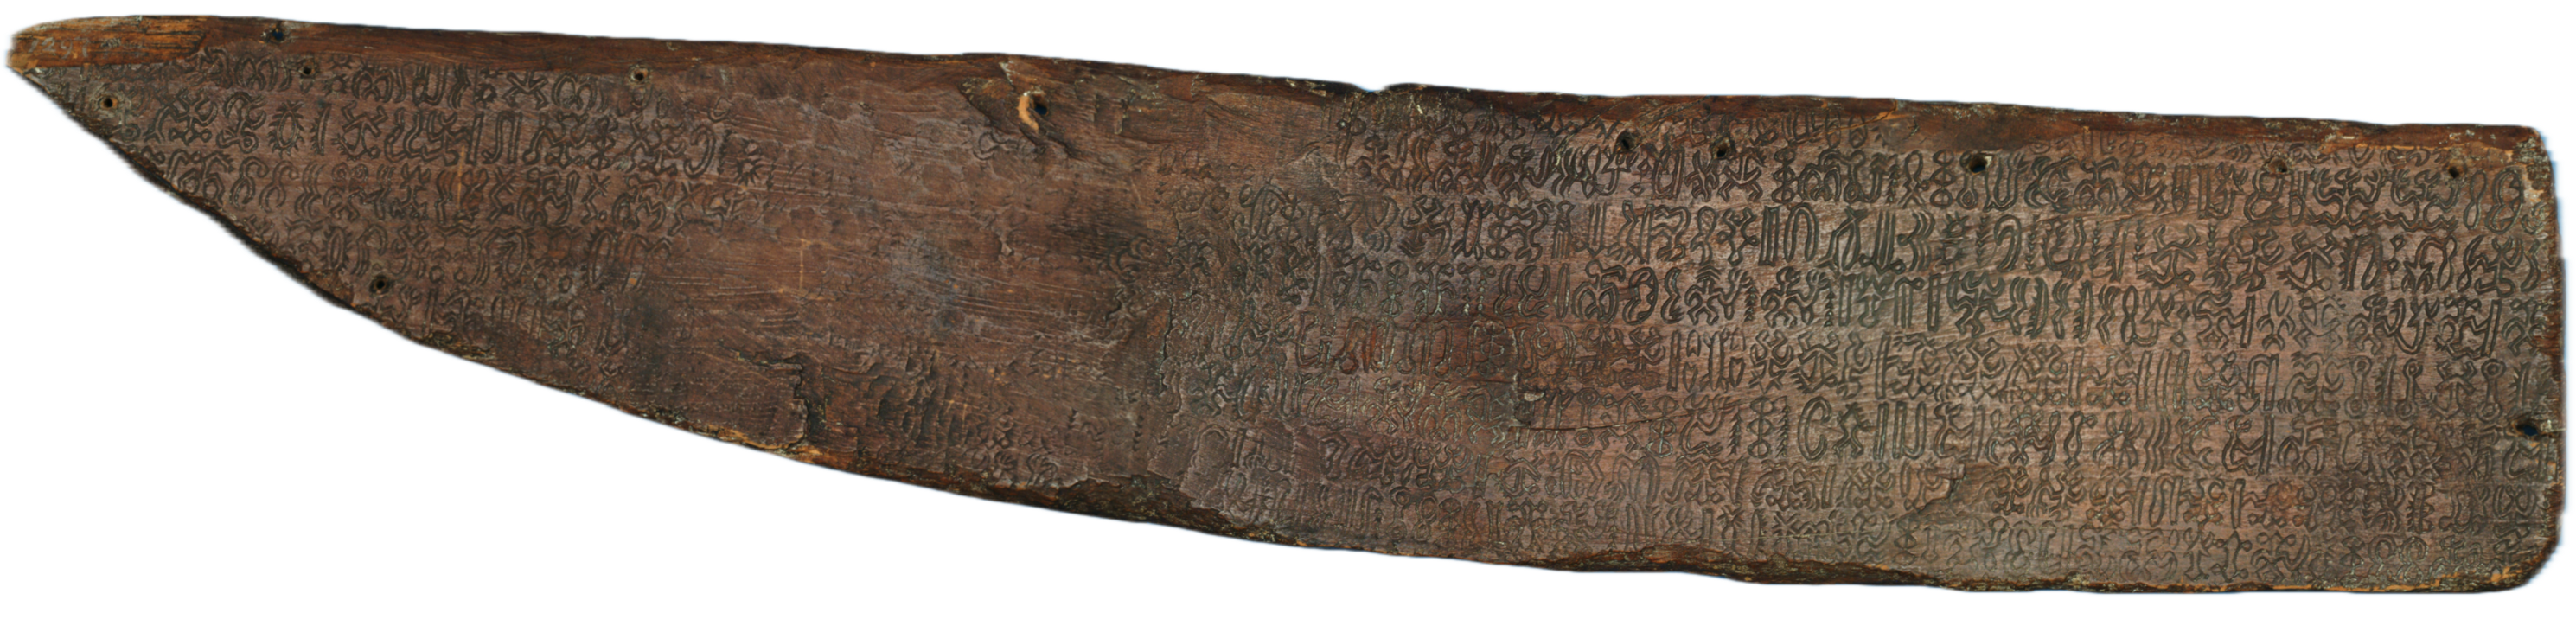
\includegraphics[width=0.9\textwidth]{fig_rongo_g_washington.png}
\caption{\textbf{Rongo Rongo Great Washington Tablet.} Images created by the Smithsonian and compliled by .}
\label{fig_rongo_g_washington}
\end{figure}

\begin{figure}[H]
\centering
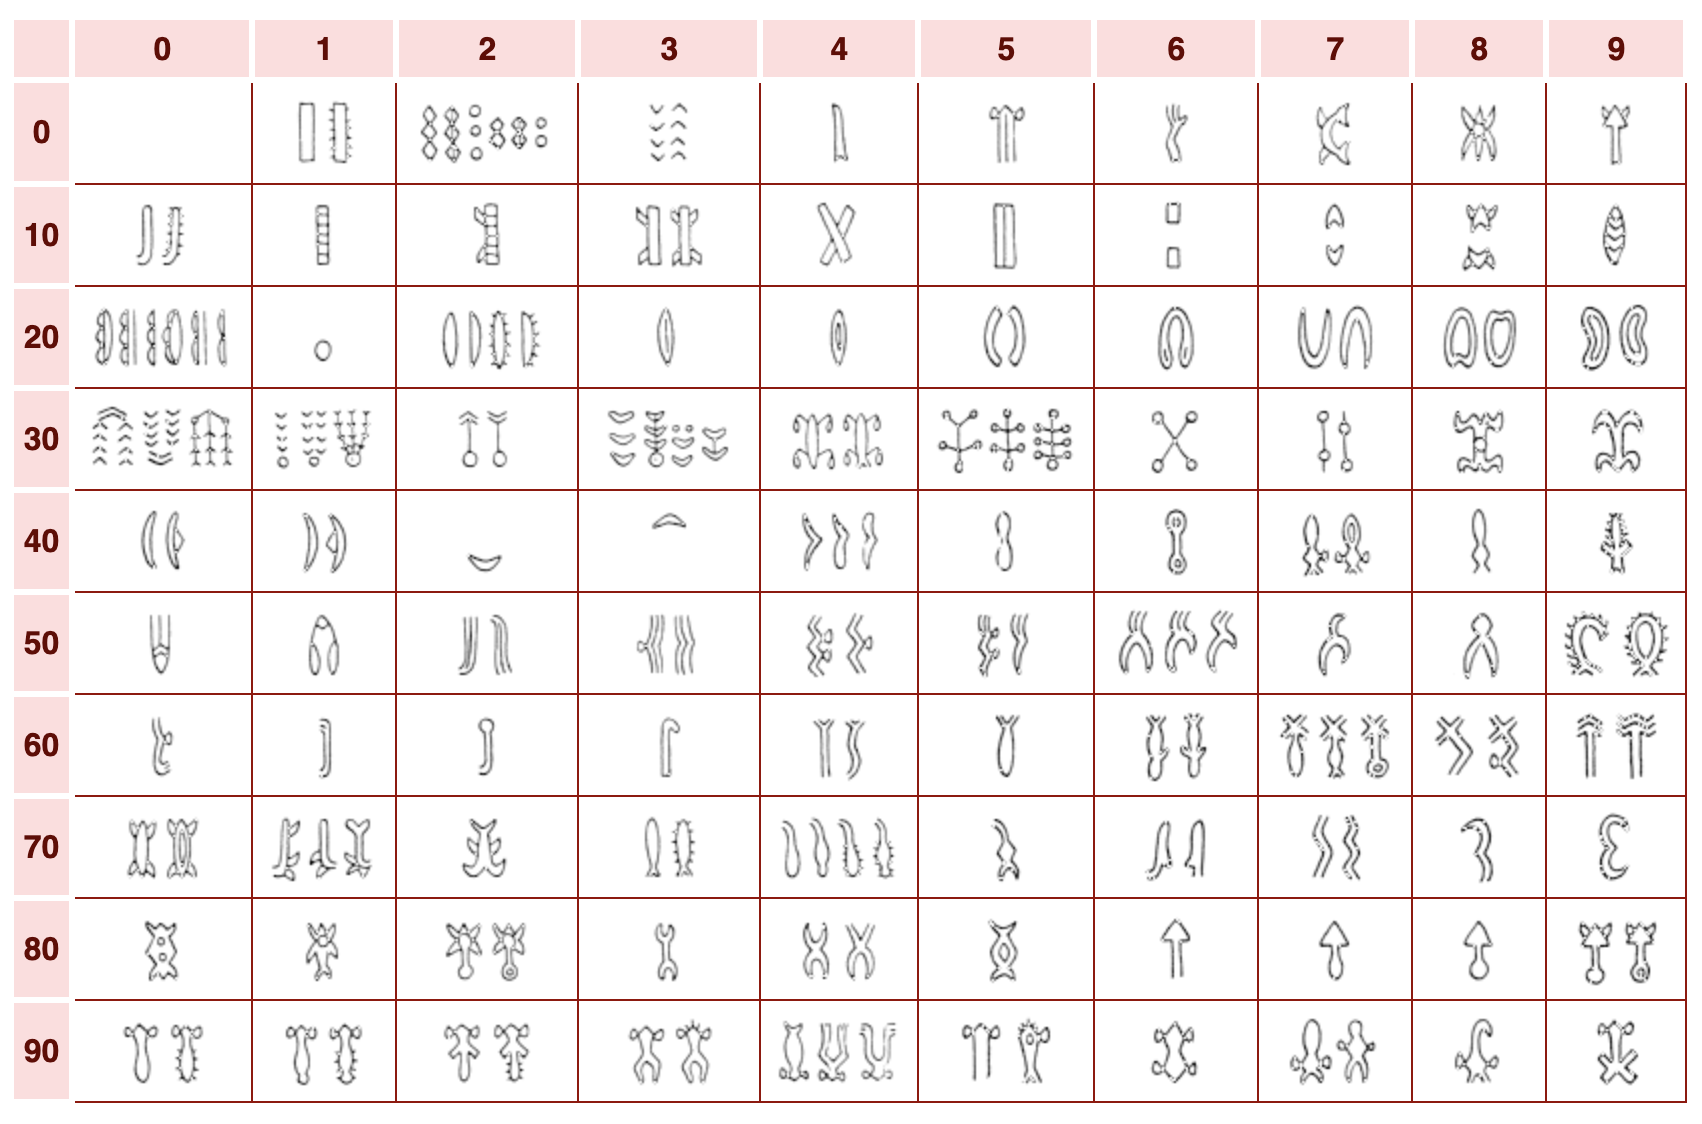
\includegraphics[width=0.9\textwidth]{fig_glyphs_example.png}
\caption{\textbf{Rongo Rongo Glyph Examples.} TODO.}
\label{fig_glyphs_example}
\end{figure}

Written in serpentine order sequenced in this order. TODO: consider left to right and right to left for both.  does it matter?  Could just say we assume temporality and were able to observe the message.  this would not be the case in a alien society reading our space craft plates. 
\subsection{Linear A}
A logosyllabic writing system
Written left to right, but some right to left and sometimes boustrophedon. In boustrophedon alternate lines of writing are reversed similar in directionality as an ox turns whiel plowing. \cite{}
%  (βοῦς, στροφή, βουστροφηδόν. Liddell, Henry George; Scott, Robert; A Greek–English Lexicon at the Perseus Project

 Emma Bennett created a signory and numbering system in 1964 \cite{}
% Bennett, E. L. Jr., "Mycenaean Studies Proceedings of the Third International Colloquium for Mycenaean Studies held at 'Wingspread', 4—8 September 1961", ed. Madison: University of Wisconsin Press, 1964

The entire linear A corpus contains around 1400 inscriptions with 7400 symbols. An additional 1100 objects are too poorly preserved to be readable and are not counted as part of this corpus.\cite{}
% Salgarella, Ester (2025). Writing in Bronze Age Crete: "Minoan" Linear A. Cambridge University Press. ISBN 9781009520027.

Most Linear A writing has been found on the island of Crete and the Aegean islands for place and religious writings. The artifacts were written on clay, stone, gold, jewelry, and pottery.  \cite{}
% Salgarella, Ester (2025). Writing in Bronze Age Crete: "Minoan" Linear A. Cambridge University Press. ISBN 9781009520027.

\begin{figure}[H]
\centering
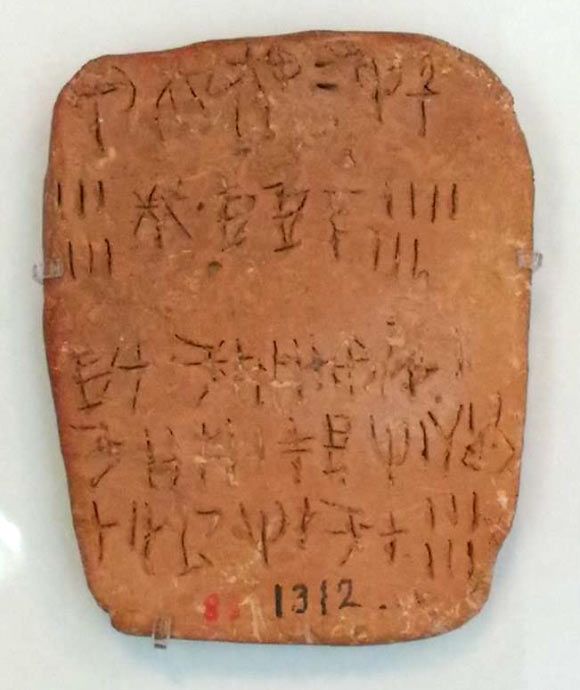
\includegraphics[width=0.9\textwidth]{fig_9329-Linear-A-Script.jpg}
\caption{\textbf{Minoan clay tablet.} Clay tablet on display at the Archaeological Museam of Heraklion inscribed with Linear A. Image credit: Ester Salgarella.}
\label{fig_linear-A-Script}
\end{figure}

The data used in this paper was sourced directly from Robert Hogan's Linear A Explorer which is a visulaizaiton tool for exploring the Linear A Language. \cite{}
https://lineara.xyz/

The Linear A Explorer uses images and transcriptions from Luis Godart and Jean-Pierre Olivier \cite{}
% [Louis Godart and Jean-Pierre Olivier](https://bit.ly/2H6Ohwe) in 1970 and of the 
as well as the tabulations by George Douros. \cite{}
\cite{}
% [tabulation and interpretation of the inscriptions by George Douros](http://users.teilar.gr/~g1951d/).

%%%%%%%%%%%%%%%%%%%%%%%%%%%%%%%%%%%%%%%%%%%%%%%%%%%%%%%%%%%%%%%%%%%%%%%%%%%%%%%%%%%
% Methodology and rationale 
%%%%%%%%%%%%%%%%%%%%%%%%%%%%%%%%%%%%%%%%%%%%%%%%%%%%%%%%%%%%%%%%%%%%%%%%%%%%%%%%%%%
\section{Methodology and Rationale}
\label{meth}
We apply a machine learning clustering pipeline centered around an HDBSCAN model and information-theoretic techniques as complementary methods. HDBSCAN attempts to group data points into separable clusters by evaluating multivariate similarity among informational features. HDBSCAN is especially useful in unknown languages since it creates separation without requiring labels or a predetermined number of clusters. Information-theoretic measures summarize corpus properties such as uncertainty, redundancy, and properties relevant to decipherability. Shannon entropy measure the uncertainty in the distribution while redundancy reflects predictable or repeatable structure. Both approaches distinguish patterns that can be inferred from the data without linguistic or archeological interpretations. 

Data transformation techniques used in this paper require the symbols of both the Rongorongo and Linear A scripts to be analyzed as individual symbols (uni-grams) and sequences of symbols (n-grams). When a technique or data processing stage uses both uni-grams and n-grams we refer to them collectively as observations.

\subsection{Data Preparation}
\subsubsection{Tokenization} *** NOT IN CODE YET ***
Each individual symbol was tokenized by simple indexing. Each visibly atomic symbol identified by prior research such as \cite{} \cite{} \cite{} is assumed to be the atomic element of information or symbol. Each symbol is simply a distinct indexed item such as 001 for Rongorongo or *** INSERT COOL glyph *** in the case of Linear A. 

\subsubsection{Sequence Construction}
TODO: Reference why this is used in cryptoanalysis and why it might apply here. 
Each corpus is sequenced as one long single sequence. No boundary or gap tokens are used as these would require an assumption of knowledge on the underlying structure of the communication. This places empty spaces on the same informational level as symbols.
Let the resulting ordered token sequence be
\[
X = (x_1,x_2,\ldots,x_L),
\]where \(L\) is the number of tokens in the corpus.

\subsubsection{Frequency Rank Normalization} *** NOT IN CODE YET ***
Each corpus is frequency rank normalized independently before the corpora are merged. Let \(\mathcal{S}_c\) denote the set of observed symbols in corpus \(c\), with corpus frequency \(f_c(s)\) calculated. Signs are then ordered from most to least frequent. Tied frequencies are assigned their mean rank.

Since the corpora contain different numbers of symbols, ranks are normalized with:
\[
\rho_c(s)=\frac{r_c(s)-1}{|\mathcal{S}_c|-1},
\]
where \(r_c(s)\) is the frequency rank of 
symbol \(\left|\mathcal{S}_c\right|\). \(\rho_c(s)=0\) represents the most frequent sign, while values approaching \(1\) represent increasingly rare signs.

Frequency rank normalization removes sign identity and gives the two scripts a shared feature space. This shared feature space allows HDBSCAN to compare patterns of relative symbol frequency and prevents the algorithm from separating the corpora merely based on different symbol inventories. 

\subsection{Machine Learning with HDBSCAN}
HDBSCAN pipeline consists of seven separate stages. Corpus Ingestion, TF-IDF Vectorization and UMAP Dimensionality Reduction prepare the data for the HDBSCAN algorithm. The HDBSCAN algorithm analyzes the data to form groups by evaluating the relative density and proximity of the data points. Topic extraction supports interpretation of resulting clusters and 3D Projection prepares the HDBSCAN output for 3 dimensional visualization. The following paragraphs describe each step of the process.

\begin{figure}[H]
\centering
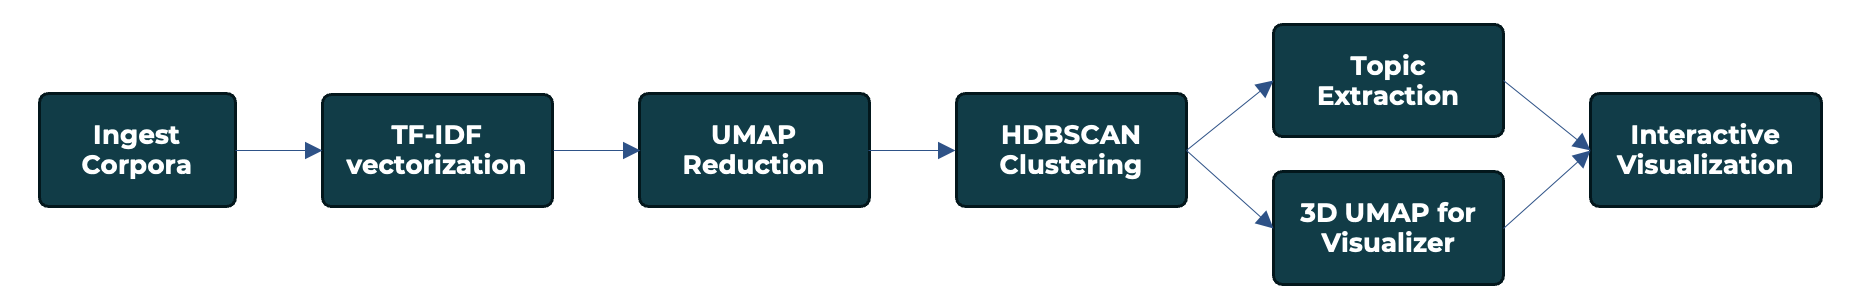
\includegraphics[width=0.9\textwidth]{fig_HDBSCAN Pipeline.png}
\caption{\textbf{HDBSCAN Pipeline.} HDBSCAN pipeline showing Corpus Ingestion, TF-IDF Vectorization, UMAP Dimensionality Reduction, HDBSCAN Clustering, Topic Extraction, Three Dimensional Projection, and Interactive Visualization used in the analysis.}
\label{fig_HDBSCAN_pipeline}
\end{figure}

\subsubsection{Corpus Ingestion}
Rongorongo and Linear A transcriptions are ingested into the pipeline and merged into a single document collection.  Source identities are kept for subsequent evaluation and visualization but are not used to guide clustering or other algorithms. 

\subsubsection{Vectorization}
Each observed symbol is converted into a vector based on uni-gram and bi-gram features using TF-IDF.  Vectorization was restricted to bi-grams due to the relatively low amount of data available in order to ensure *** JUSTIFY it kept erroring somehow ***..  TF-IDF emphasizes terms that are important in the sequence of text yet relatively uncommon in the corpus.  

\subsubsection{Dimensioality Reduction}
Dimensionality reduction was performed using the UMAP algorithm. This reduces the high dimensionality resulting from the TF-IDF vectorization into 42 dimensions *** JUSTIFY ***. Cosine distance was chosen because it compensates for document size by length normalizing the vectors to unit vectors. 

\subsubsection{HDBSCAN Clustering}
Clustering is performed by HDBSCAN. The algorithm searches the 42-dimensional space for stable regions of high density. HDBSCAN was chosen because it does not require the number of clusters to be selected before hand. A minimum cluster size of 50 *** JUSTIFY *** was used. Once the model identifies the stable regions of high density is assigns each symbol or sequence of symbols to a stable cluster. If the observation is not a fit for one of the clusters it is labeled as noise. 

\subsubsection{Topic Extraction}
Each cluster is then labeled with a topic using the five terms with the greatest TF-IDF weight among it's observations. This helps identify the symbols or sequences of symbols best represent the cluster. 

\subsubsection{3D Projection}
In order to display the 42 dimensions used to cluster the symbols in human readable form UMAP was once again used for dimensionality reduction. The 42 dimensions projected onto a 3-dimensional space superimpose the higher dimensional space. As a consequence the displayed coordinates are illustrative and are not the actual space used for clustering.

\subsubsection{Interactive Visualization}
The visualization shown is a static representation of a interactive visualization that can be used to display the observations by cluster, characteristic terms, and a preview of the corresponding observation. 

\subsection{Information Theoretical}
The informaiton theoretical pipline starts with raw data as defined in \ref{data}. n-grams of orders 1-4 ***JUSTIFY*** are prepared from this raw data. Each data set is analyzed from an frequency, 

\subsubsection{N-gram Construction}
Overlapping \(n\)-grams were generated for \(n \in \{1,2,3,4\}\). The \(i\)-th \(n\)-gram is defined as
\[
g_i^{(n)} = (x_i,x_{i+1},\ldots,x_{i+n-1})
\]
where where \(x_i\) denotes the token at position \(i\) in a sequence of length \(L\), and \(i \in \{1,\ldots,L-n+1\}\).

The tokens in each \(n\)-gram were joined with hyphens providing a serialized representation of each sequence. 

\subsubsection{Frequency estimation}
Post n-gram construction frequency estimation is once again employed. For each value of \(n\), the the count, \(c\), of every distinct n-gram is calculated. If \(c_j\) is the frequency of the \(j\)-th distinct n-gram then its probability of occurrence is estimated with 
\[
p_j = \frac{c_j}{T_n}.
\]
Where \(T_n\) is the total number of all \(n\)-grams in the set.

If we let \(K_n\) is the number of distinct \(n\)-grams then corpus diversity can be summarized calculating the proportion of unique observations for each \(n-gram\) set
\[
Q_n = \frac{K_n}{T_n}.
\]
resulting in a set of proportions between 0 and 1 with higher values of \(Q_n\) indicating more rare occurrences of that \(n-gram\) sequence and lower values indicating higher repetition. 

\subsubsection{Entropy and Redundancy}
The Shannon entropy of each \(n-gram\) set was calculated in bits using methods outlined in \cite{}
\[
H_n = -\sum_{j=1}^{K_n} p_j \log_2 p_j.
\]
The max potential entropy in the \(n-gram\) set is defined as the entropy of a uniform distribution containing the same number of distinct symbols: 
\[
H_{n,\max} = \log_2 K_n.
\]
Normalized redundancy was calculated by first calculating absolute redundancy:
\[
D_n = H_{n,\max}-H_n,
\] and dividing by the maximum possible redundancy:
\[
R_n(D_n)=\frac{D_n}{H_{n,\max}}
\]
In this way \(D_n\) measures the redundancy as departures from uniformity in bits per \(n\)-gram and \(R_n\) shows the same departure from uniformity as a proportion of maximum entropy following the work of \cite{}. 

\subsubsection{Keyspace, Unicity Distance and Theoretical Decipherability Margin}
Possible key space and unicity distance are calculated to determine if the set of \(n\)-grams contains enough information to make a theoretical decipherment possible. 

A key space is the set of all possible keys in a cypher model. In this model the key space is all possible permutations of the \(n-gram\) sets and is calculated 
\[
|\mathcal{K}_n| = K_n!,
\]and the corresponding key-space size in bits is
\[
B_n = \log_2(K_n!).
\]
Observed unicity distance for the \(n-gram\) set is then calculated by 
\[
U_n = \frac{B_n}{D_n}.
\]
The resulting values from the unicity distance calculation estimates the number of \(n-gram\) observations required for redundancy to overcome uncertainty in the substitution key and contain enough information to identify a unique mapping. 

Finally the theoretical decipherability margin was calculated by subtracting the unicity distance \(U_n\) from the total number of \(n-grams\) \(T_n\) in the set. A positive margin indicates the corpus, as sequenced \(n-gram\) sets, is estimated to contain sufficient information to identify the key as unique. It therefore indicates informational-theoretic decipherability. It does not guarantee the key can be recovered computationally, but that it is possible to be accomplished given the assumptions inherent in the data preparation. 

%%%%%%%%%%%%%%%%%%%%%%%%%%%%%%%%%%%%%%%%%%%%%%%%%%%%%%%%%%%%%%%%%%%%%%%%%%%%%%%%%%%
% results
%%%%%%%%%%%%%%%%%%%%%%%%%%%%%%%%%%%%%%%%%%%%%%%%%%%%%%%%%%%%%%%%%%%%%%%%%%%%%%%%%%%
\section{Analysis and Results} 
\label{anal_results}
TODO
%%%%%%%%%%%%%%%%%%%%%%%%%%%%%%%%%%%%%%%%%%%%%%%%%%%%%%%%%%%%%%%%%%%%%%%%%%%%%%%%%%%
% Discussion
%%%%%%%%%%%%%%%%%%%%%%%%%%%%%%%%%%%%%%%%%%%%%%%%%%%%%%%%%%%%%%%%%%%%%%%%%%%%%%%%%%%
\section{Discussion and Future Work}
\label{discussion}

The methods in this paper cannot decipher the meaning or linguistic composition of an unknown symbolic system. Instead they determine if the available data contain non-random regularities and what scale those regularities happen. It can also be used to determine if the corpus is of sufficient size and non-random enough to support more specific analysis. 

May be worth attempting to read un-readable Linear A scripts since the only \(1-gram\) set has enough information to be theoretically decipherable. Since the Linear A script is known to have complex symbols combined via ligature \cite{} 
% Tomas, Helena (2012). "Cretan Hieroglyphic and Linear A". In Cline, Eric (ed.). The Oxford Handbook of the Bronze Age Aegean. Oxford University Press. pp. 113–125. doi:10.1093/oxfordhb/9780199873609.013.0026. ISBN 978-0199873609.

it is likely the true decipherablility requires more information than the \(1-gram\) sequense implies. 
%%%%%%%%%%%%%%%%%%%%%%%%%%%%%%%%%%%%%%%%%%%%%%%%%%%%%%%%%%%%%%%%%%%%%%%%%%%%%%%%%%%
% appendix
%%%%%%%%%%%%%%%%%%%%%%%%%%%%%%%%%%%%%%%%%%%%%%%%%%%%%%%%%%%%%%%%%%%%%%%%%%%%%%%%%%%
\newpage 
\appendix
\section{TODO}
\label{TODO}

\begin{table}[H]
\centering
\begin{tabular}{p{1.2cm} p{7.5cm} p{3.5cm}}
 \hline
 \rowcolor[gray]{0.95}
 \textbf{Year} & \textbf{Title} & \textbf{TODO} \\ \hline
 2001 & Astronomy and Astrophysics for the New Millennium & Astrophysics \\
 \rowcolor[gray]{0.97}
 2003 & The Sun to the Earth—and Beyond: A Decadal Research Strategy in Solar and Space Physics & Heliophysics \\
 2003 & New Frontiers in the Solar System: An Integrated Exploration Strategy & Planetary  Science \\
 \rowcolor[gray]{0.97}
 2007 & Earth Science and Applications from Space: National Imperatives for the Next Decade and Beyond & Earth Science \\
\end{tabular}
\caption{Decadal Surveys Used in Analysis }\label{tab:Decadals_used}
\end{table}

\section{TODO2}
\label{TODO2}
This section details TODO

\begin{description}
 \item[TODO1:] Follow a \texttt{yyyy-DS-Category-\#\#\#\#.pdf} format where \texttt{\#\#\#\#} is the National Academies document number. \texttt{DS} is used to categorize all Decadal Surveys. \texttt{MA} replaces \texttt{DS} for Midterm Assessments, and \texttt{SP} is used for the Special Publication in 2015 that identified lessons learned.
 
 \item[TODO2:] Follow a \texttt{yyyy\_SSP\_Nasa\_File\_Name.pdf} format. \texttt{SSP} represents Science mission directorate Science Plans. This is replaced with \texttt{AD} to indicate Additional Documentation, \texttt{NSP} to indicate NASA Science Plan, or \texttt{AD} to indicate additional documentation present on the SMD website.
\end{description} 


%% Bibliography
\bibliographystyle{elsarticle-num} 
\bibliography{master.bib}

\end{document}
